\documentclass[oneside, 11pt]{article}

\usepackage[T1]{fontenc}
\usepackage[utf8]{inputenc}
\usepackage[dutch]{babel}

\usepackage{fouriernc}
\usepackage[detect-all, load-configurations=binary,
            separate-uncertainty=true, per-mode=symbol,
            retain-explicit-plus, range-phrase={ tot }]{siunitx}

\usepackage{setspace}
\setstretch{1.2}

\setlength{\parskip}{\smallskipamount}
\setlength{\parindent}{0pt}

\usepackage{geometry}
\geometry{marginparwidth=0.5cm, verbose, a4paper, tmargin=3cm, bmargin=3cm, lmargin=2cm, rmargin=2cm}

\usepackage{float}

\usepackage[fleqn]{amsmath}
\numberwithin{equation}{section}
\numberwithin{figure}{section}

\usepackage{graphicx}
\graphicspath{{Figures/}}
\usepackage{subfig}

\usepackage{tikz}
\usetikzlibrary{plotmarks}

\usepackage{fancyhdr}
\pagestyle{fancy}
\fancyhf{}
\rhead{\thepage}
\renewcommand{\footrulewidth}{0pt}
\renewcommand{\headrulewidth}{0pt}

\usepackage{relsize}
\usepackage{xspace}
\usepackage{url}

\newcommand{\figref}[1]{Figuur~\ref{#1}}

\newcommand{\hisparc}{\textsmaller{HiSPARC}\xspace}
\newcommand{\kascade}{\textsmaller{KASCADE}\xspace}
\newcommand{\sapphire}{\textsmaller{SAPPHiRE}\xspace}
\newcommand{\jsparc}{\textsmaller{jSparc}\xspace}
\newcommand{\hdf}{\textsmaller{HDF5}\xspace}
\newcommand{\aires}{\textsmaller{AIRES}\xspace}
\newcommand{\csv}{\textsmaller{CSV}\xspace}
\newcommand{\python}{\textsmaller{PYTHON}\xspace}
\newcommand{\corsika}{\textsmaller{CORSIKA}\xspace}
\newcommand{\labview}{\textsmaller{LabVIEW}\xspace}
\newcommand{\daq}{\textsmaller{DAQ}\xspace}
\newcommand{\adc}{\textsmaller{ADC}\xspace}
\newcommand{\adcs}{\textsmaller{ADC}s\xspace}
\newcommand{\Adcs}{A\textsmaller{DC}s\xspace}
\newcommand{\hi}{\textsc{h i}\xspace}
\newcommand{\hii}{\textsc{h ii}\xspace}
\newcommand{\mip}{\textsmaller{MIP}\xspace}
\newcommand{\hisparcii}{\textsmaller{HiSPARC II}\xspace}
\newcommand{\hisparciii}{\textsmaller{HiSPARC III}\xspace}
\newcommand{\pmt}{\textsmaller{PMT}\xspace}
\newcommand{\pmts}{\textsmaller{PMT}s\xspace}

\DeclareSIUnit{\electronvolt}{\ensuremath{\mathrm{e\!\!\:V}}}

\DeclareSIUnit{\unitsigma}{\ensuremath{\sigma}}
\DeclareSIUnit{\mip}{\textsmaller{MIP}}
\DeclareSIUnit{\adc}{\textsmaller{ADC}}

\DeclareSIUnit{\gauss}{G}
\DeclareSIUnit{\parsec}{pc}
\DeclareSIUnit{\year}{yr}



\title{Detector bouw}
\author{A.P.L.S. de Laat, J.G. Oldenziel} 
\docinstallatie{1}{DB}
\version{1.0}

\begin{document}

\maketitle

\section{Detector bouw handleiding}

Dit document beschrijft de stappen die nodig zijn bij het
maken van een \hisparc detector. Een detector bestaat uit een
scintillator, een lichtgeleider met aansluitblokje en een fotoversterker
buis (Photo Multiplier Tube (\pmt)). De lichtgeleider wordt op de
scintillator gelijmd en het aansluitblokje op de lichtgeleider. Nadat de
lijm gedroogd is, wordt het geheel ingepakt in aluminiumfolie en
vijverfolie. De \pmt wordt geijkt en op het aansluitblokje geplakt met
optische tape. De aangesloten \pmt wordt tot slot ook lichtdicht verpakt. 


\section{Materiaal lijst}

Dit zijn de materialen waar een detector uit bestaat:

\begin{itemize}
    \item 2 Scintillatoren
    \item 2 Lichtgeleiders
    \item 2 Aansluitblokjes
    \item 2 Fotoversterkerbuizen (\pmt, model 9125B)
    \item Lijm (EJ 500)
    \item Optische tape
    \item Aluminiumfolie (dik en dun)
    \item Zwart lichtdicht folie
    \item Plakband (Scotch)
    \item Zwarte tape
    \item 8 Houten spalkjes
\end{itemize}

En dit zijn de andere benodigdheden:

\begin{itemize}
    \item Handschoenen
    \item Schuimblokken
    \item Anti-statische doek
    \item Alcohol
    \item Tissues
    \item Optische doekjes
    \item Schuurpapier (type 500 of 600, waterbestendig)
    \item Tape die geen lijmresten achterlaat
    \item Schilders tape
    \item Mesje en schaar
    \item Vacuümpomp
    \item Roerstaafje
    \item Digitale weegschaal (\SI{0.1}{\gram} nauwkeurig)
    \item Lijmmal
    \item Lijmklemmen
\end{itemize}


\section{Voorbereiding scintillatorplaat, lichtgeleider en aansluitblokje}

Voordat de verschillende onderdelen gelijmd kunnen worden, moeten de lijmoppervlakken voorbereid worden. Als eerste moeten deze oppervlakken worden opgeruwd. De te verlijmen oppervlakken van de scintillator en de lichtgeleider worden vlak geschuurd. Dit wordt ook gedaan met de te verlijmen oppervlakken van de lichtgeleider en het aansluitblokje. Vlakke oppervlakken dragen bij aan een goede aansluiting zonder ingesloten luchtbelletjes. Het schuren zorgt ook dat de lijm beter hecht aan het materiaal. 


\subsection{Schuren van lijm oppervlak scintillatorplaat}

\textbf{Let op!} Altijd handschoenen aan wanneer je met de
scintillatorplaat werkt! Het vet op je handen tast het oppervlak aan! Zorg ook voor een schone werkomgeving, maak de tafel waar je op gaat werken schoon voor je begint.

\begin{enumerate}
    \item Leg een stuk schuimblok op de tafel om de plaat op te leggen.
    \item Haal ongeveer \SI{5}{\centi\meter} van het beschermingspapier,
    dat om de scintillatorplaat zit, los aan de kant waar de lichtgeleider
    komt.
    \item Schuur de scintillatorplaat nat met type 500 of 600 watervast
    schuurpapier:
    \begin{enumerate}
        \item Bevestig hiervoor het schuurpapier met dubbelzijdig
        plakband op een vlak houtblokje.
        \item Druk het blokje met schuurpapier voorzichtig tegen het natte oppervlak,
        als je het loslaat blijft het hangen.
        \item Schuur deze kant vlak met water. Zorg dat het schuurblokje vlak tegen het
        oppervlak blijft. Ook nu moet het blokje blijven hangen als je het loslaat. Let vooral
        op bij de hoeken, je gaat daar gemakkelijk fout.
        \item Maak lange schuurbewegingen over de hele lengte,
        concentreer je niet steeds op één stukje.
        \item Ga door tot het oppervlak goed geschuurd is. Het is overal even mat
        geworden.
    \end{enumerate}
    \item Maak het te lijmen oppervlak schoon met een tissue en water.
    Daarna met een optische doekje en alcohol.
    \item Plak de rand van het te lijmen oppervlak over
    \SI{5}{\centi\meter} breedte zeer nauwkeurig af met speciale
    kwaliteit tape, dat geen lijmresten achterlaat, zoals te zien in
    \figref{fig:rand_afplakken}.
    \item Maak op deze speciale tape anti-lekgootjes met dubbel
    papierplakband (schilderstape). Zorg ervoor dat de gootjes niet om
    kunnen klappen.
    \item Maak de rand schoon met een anti-statische doek.
    \item Zet de scintillatorplaat in de mal. Let op vlakke aansluiting,
    niet te sterk klemmen. Let ook op de lekgootjes.
\end{enumerate}

\begin{figure}
    \centering
    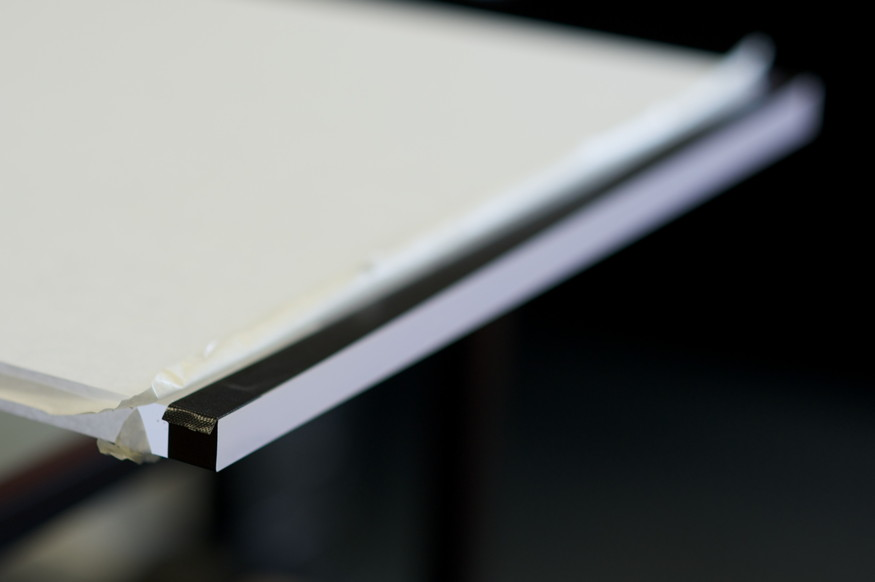
\includegraphics[width=0.47\linewidth]{rand_afplakken}
    \caption{Het afplakken van de randen zodat er geen lijm op het
             materiaal komt waar het niet moet komen.}
    \label{fig:rand_afplakken}
\end{figure}


\subsection{Schuren van de lichtgeleider}

\begin{enumerate}
    \item Plaats de lichtgeleider ook op een schuimblok op de tafel.
    \item Haal aan beide zijden een stuk van het beschermfolie af.
    \item Schuur de lichtgeleider nat aan beide kanten met watervast
    schuurpapier type 500 of 600, net als de scintillator.
    \item Maak aan bovenkant van de lichtgeleider (smalle deel) rondom
    een gootje van dubbel papierplakband.
\end{enumerate}

\begin{figure}
    \centering
    \subfloat[]{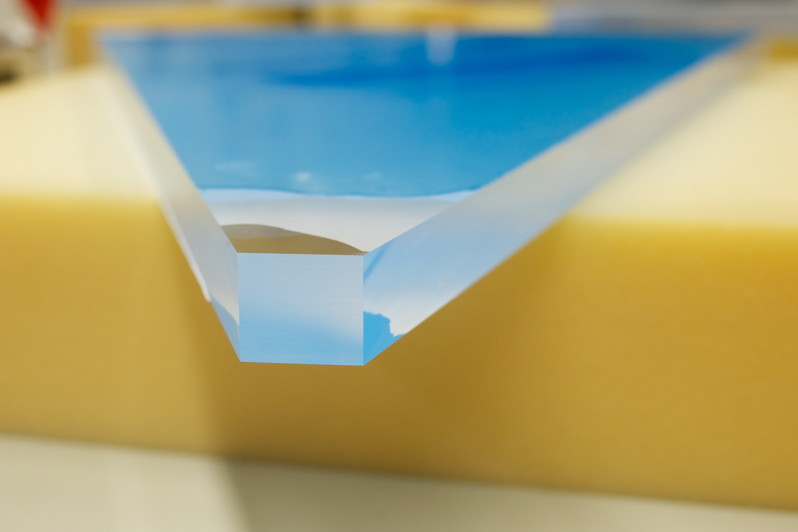
\includegraphics[width=0.47\linewidth]{lichtgeleider}
                \label{fig:lichtgeleider}}
    \subfloat[]{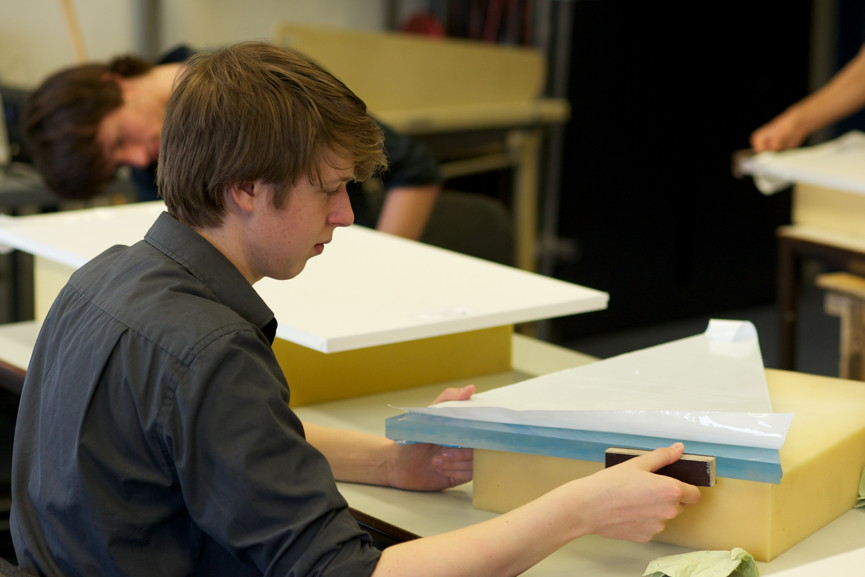
\includegraphics[width=0.47\linewidth]{schuren}
                \label{fig:schuren}}
    \caption{Het schuren van de lichtgeleiders en scintilatoren.}
\end{figure}


\subsection{Schuren van het aansluitblokje}

In \figref{fig:blokjes} zijn een aantal aansluitblokjes te zien.

\begin{enumerate}
    \item Schuur de kant van het aansluitblokje waar het mee aan de
    lichtgeleider komt (de vierkante kant). De andere kant niet!
    \item Het blokje is zo klein dat het handiger is om het (natte)
    schuurpapier op tafel te leggen en het blokje er overheen te bewegen.
    \item Ga door tot het blokje goed geschuurd is, maak deze daarna ook
    schoon met een optische doekje en alcohol.
\end{enumerate}

\begin{figure}
    \centering
    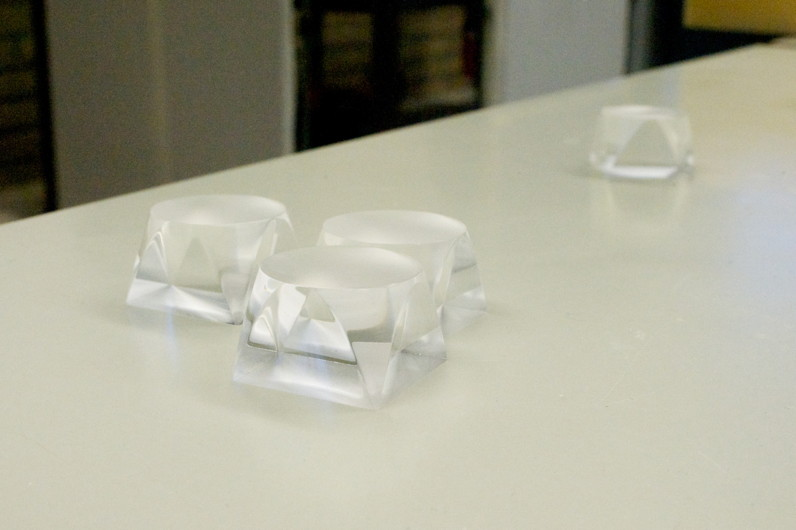
\includegraphics[width=0.47\linewidth]{blokjes}
    \caption{De aansluitblokjes tussen de lichtgeleider en de \pmt.}
    \label{fig:blokjes}
\end{figure}


\section{Lijmprocedure}

Wanneer de te lijmen onderdelen voorbereid zijn, kan het lijmen beginnen.

\begin{enumerate}
    \item Leg de lijmklemmen klaar bij de montagemal.
    \item Oefen de lijmprocedure eerst met water door de lichtgeleider
    langs de mal op de scintillatorplaat te laten zakken. Eerst wordt in een hoek
    contact gemaakt. Daarna draait de lichtgeleider op de scintillator. Je ziet
    eventueel dat belletjes opzij bewegen. Oefen net zo lang tot je de techniek
    beheerst.
    \item Leg na het oefenen de lichtgeleider weer op tafel en maak de
    oppervlakken goed droog door deppen.
    \item Maak de twee componenten optische lijm aan:
    \begin{enumerate}
        \item Let op: schone handen zijn belangrijk, neem zonodig nieuwe
        handschoenen
        \item Plaats een in een bekerglas op de digitale weegschaal.
        En zet de schaal weer op \SI{0}{\gram}. Noteer ook het gewicht
        van het lege bekerglas.
        \item Spuit met behulp van een plastic injectiespuit
        \SI{8}{\gram} epoxyhars EJ 500 (\SI{4}{\gram} per plaat) in het
        bekerglas.
        \item Voeg met behulp van een dunne injectiespuit druppelsgewijs
        precies \SI{2}{\gram} harder EJ 500 (\SI{1}{\gram} per plaat)
        toe. (NB: voor andere types epoxyhars kunnen andere verhoudingen
        gelden!)
        \item Verzwaar de beker aan de onderkant m.b.v. een lijmklem,
        zodat hij stevig staat en niet gemakkelijk omvalt.
        \item Meng de lijm goed door te roeren met een schoon plastic of
        glas staafje.
        \item Zet de beker in een exsiccator en zuig vacuüm tot alle
        luchtbellen verdwenen zijn. Zorg ook hier dat de beker stabiel
        staat en niet om kan vallen.
    \end{enumerate}
    \item Controleer de te lijmen oppervlakken goed en reinig ze zo
    nodig met alcohol.
    \item Breng de lijm voorzichtig aan met een roerstaaf in een
    aaneengesloten spoor op de bovenkant van de scintillatorplaat. Zoals
    in \figref{fig:lijmen}.
    \item Laat de lichtgeleider langzaam op de scintillatorplaat zakken.
    Let er tijdens het zakken goed op dat de lijmlaag een aaneengesloten
    geheel wordt.
    \item Klem de lichtgeleider vast aan de mal met de lijmklemmen,
    zoals te zien in \figref{fig:mal}. Zorg ervoor dat het oppervlak
    niet beschadigt.
    \item Breng nu voorzichtig lijm aan met een roerstaaf op de
    bovenkant van de lichtgeleider.
    \item Plak daarna het aansluitblokje op de lichtgeleider. Let erop
    dat het er goed op zit op de juiste plaats. Houd het op de plaats
    met stevig plakband zoals in \figref{fig:blokje_verankering}.
\end{enumerate}

\textbf{De lijm moet nu minstens 48 uur drogen.}

\begin{figure}
    \centering
    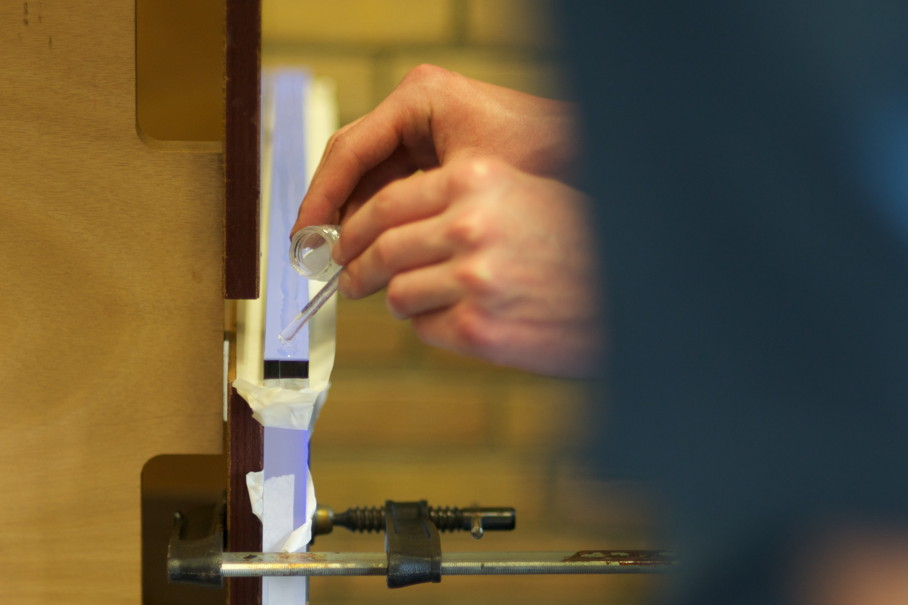
\includegraphics[width=0.47\linewidth]{lijmen}
    \caption{Het aanbrengen van de lijm met een roerstaafje.}
    \label{fig:lijmen}
\end{figure}

\begin{figure}
    \centering
    \subfloat[]{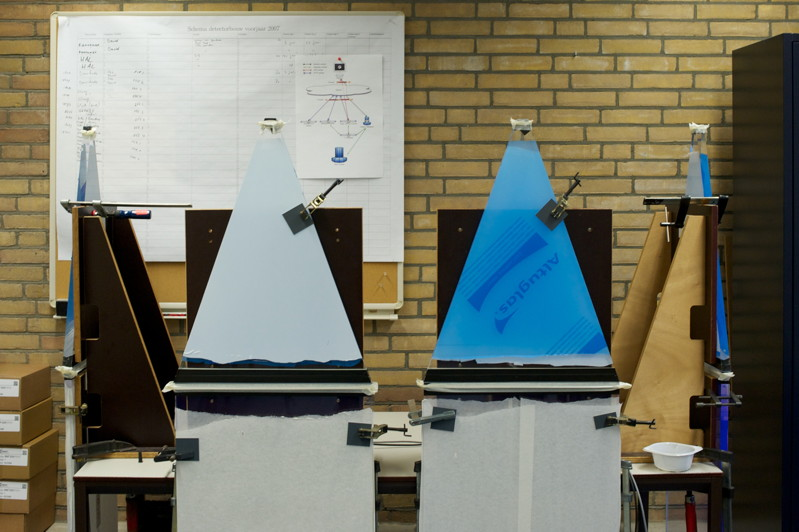
\includegraphics[width=0.47\linewidth]{mal}
                \label{fig:mal}}
    \subfloat[]{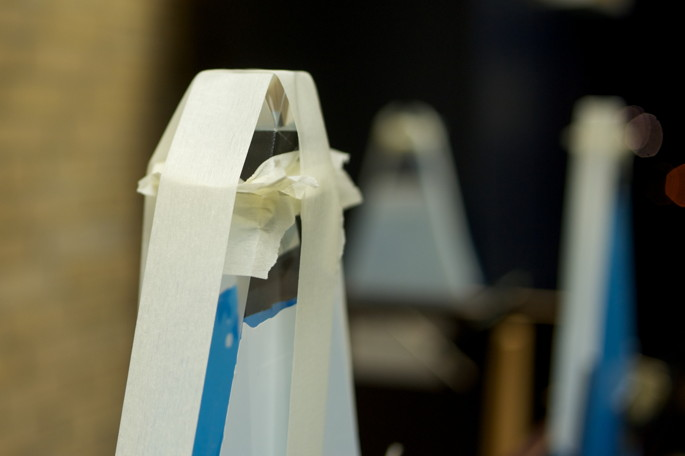
\includegraphics[width=0.47\linewidth]{blokje_verankering}
                \label{fig:blokje_verankering}}
    \caption{De gelijmde detector in de mal verankerd zodat het goed kan
             drogen. Het aansluitblokje wordt op zijn plaats gehouden
             met tape.}
\end{figure}


\section{Lichtdicht maken van de detector}

\textbf{Let op!} Handschoenen aan! Tafels goed schoon houden!

\begin{enumerate}
    \item Haal de detector uit de mal en leg hem weer op de tafel.
    Verwijder het plakband en eventuele lijmresten voorzichtig m.b.v.
    een dun en scherp mesje.
    \item Verwijder de beschermfolie van de scintillatorplaat en de
    lichtgeleider.
    \item Maak de oppervlakken schoon met een antistatische doek, en
    eventueel ook met alcohol, zie \figref{fig:poetsen_detector}.
    \item Bereid op een andere tafel het inpakken in aluminiumfolie en
    vijverfolie voor. Maak deze tafel zorgvuldig schoon om gaatjes in de
    folies te voorkomen.
    \item Meet het zwarte vijverfolie af: minstens
    \SI{120}{\centi\meter} breed en ongeveer \SI{175}{\centi\meter}
    lang, en leg het op de tafel, maak het antistatisch met het doekje.
    \item Snij van de rol dikke aluminium folie vier korte stukken af,
    vouw deze een aantal keren dubbel (zonder al te veel kreukels te
    maken in het folie).
    \item Leg deze vier stukken op het vijverfolie op de plaats van de
    hoeken van de scintillator, dit zal dienen als versteviging van de
    hoeken.
    \item Snij dun aluminiumfolie ter breedte van de rol op een lengte
    van \SI{175}{\centi\meter} af en leg dit op het vijverfolie.
    \item Leg de detector in een keer goed op het aluminiumfolie, zodat
    de hoekpunten op de verstevigingen liggen. Schuif niet met de
    detector, dan kan het aluminium folie scheuren! Zie
    \figref{fig:open_detector}.
    \item Vouw nu het aluminiumfolie aan de zijkanten om de
    scintillatorplaat. Knip het folie aan de hoeken in en vouw het en nu
    ook om de onderkant. Zorg dat dit blijft zitten door de vouwen van
    aluminium folie aan elkaar te plakken met Scotch plakband. Let op
    dat het plakband niet op de scintillator komt.
    \item Vouw het folie om de rand van de lichtgeleider en weer terug,
    zodat een rand zichtbaar wordt die kan dienen als oriëntatie bij
    het afsnijden. Snij het folie met een scherp stanleymes en een
    metalen liniaal op maat, zodat het een paar centimeter over de rand
    uit steekt.
    \item Vouw het nu weer om de lichtgeleider en gebruik ook Scotch
    plakband om dit op z'n plek te houden. 
    \item Laat aan de bovenkant een stukje van ca \SI{5}{\centi\meter}
    vrij voor de montage van folie voor \pmt.
    \item Snij op een andere tafel een nieuw stuk aluminiumfolie op maat
    af, in breedte en lengte precies passend op de detector.
    \item Leg het folie op de detector op het omgevouwen folie, en plak
    het strak af met plakband, eerst met stukjes, later met hele repen.
    Zoals in \figref{fig:aluminiumfolie_afplakken}
    \item Versterk de hoeken en scherpe randen nu met het dubbelgevouwen
    dik folie, knip dit in en vouw het om de hoeken. Bevestig dit ook
    goed met plakband. Eerst de bovenkant, en daarna de onderkant door
    voorzichtig de hele detector (inclusief vijverfolie) naar de kanten
    van de tafel te schuiven zodat je bij onderkant de hoeken ook bij de
    onderkant kan. Uiteindelijk ziet het er uit zoals in
    \figref{fig:hoek_versteviging}.
    \item Vouw nu het zwarte vijverfolie om en pak de detector lichtdicht
    in, op het aansluitblokje na zodat de \pmt nog bevestigd kan worden.
    \item Plak de zwart plastic naden drievoudig met zwart PVC plakband.
    Laat de repen PVC plakband eerst uithangen in verband met
    elasticiteit. Zorg bij het plakken dat er zo min mogelijk
    luchtbellen onder de tape blijven. Zie \figref{fig:vijverfolie_tape}.
\end{enumerate}

\begin{figure}
    \centering
    \subfloat[]{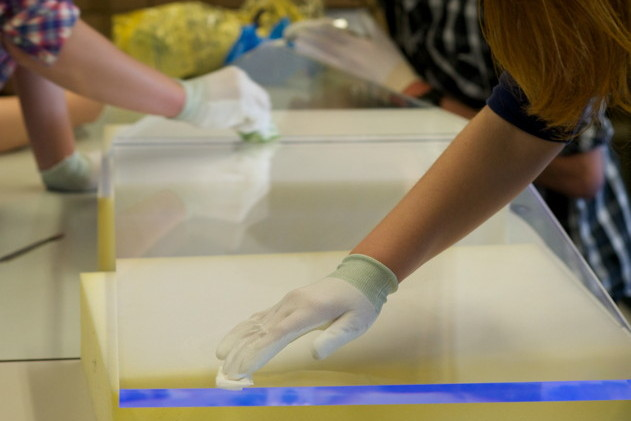
\includegraphics[width=0.47\linewidth]{poetsen_detector}
                \label{fig:poetsen_detector}}
    \subfloat[]{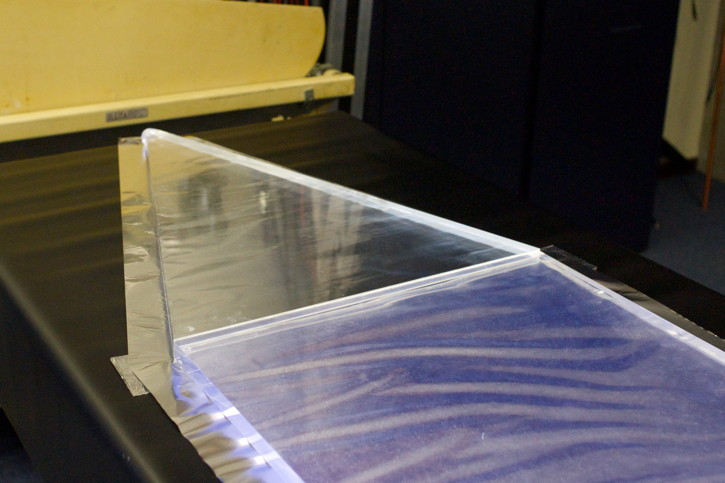
\includegraphics[width=0.47\linewidth]{open_detector}
                \label{fig:open_detector}}
    \caption{De detector goed met alcohol poetsen voor het plaatsen op
             het aluminiumfolie.}
\end{figure}

\begin{figure}
    \centering
    \subfloat[]{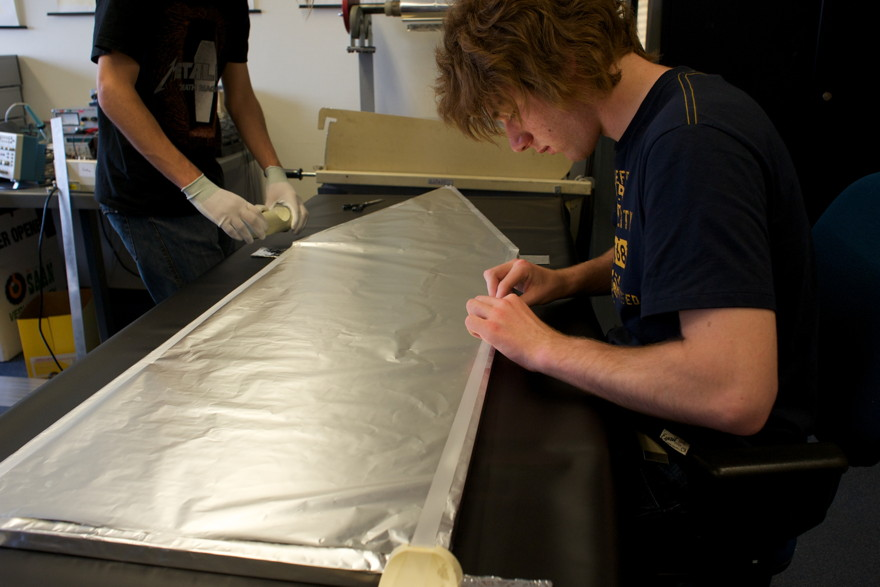
\includegraphics[width=0.47\linewidth]{aluminiumfolie_afplakken}
                \label{fig:aluminiumfolie_afplakken}}
    \subfloat[]{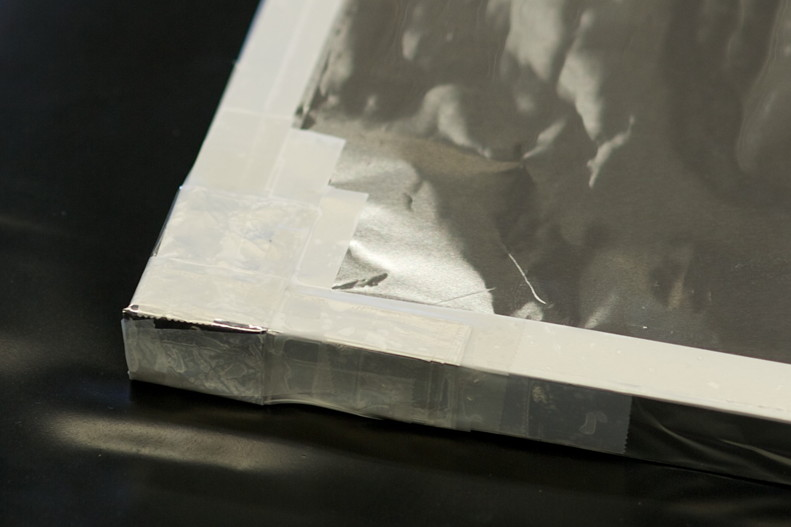
\includegraphics[width=0.47\linewidth]{hoek_versteviging}
                \label{fig:hoek_versteviging}}
    \caption{Inpakken van de detector. Verstevigde hoeken goed vast geplakt.}
\end{figure}

\begin{figure}
    \centering
    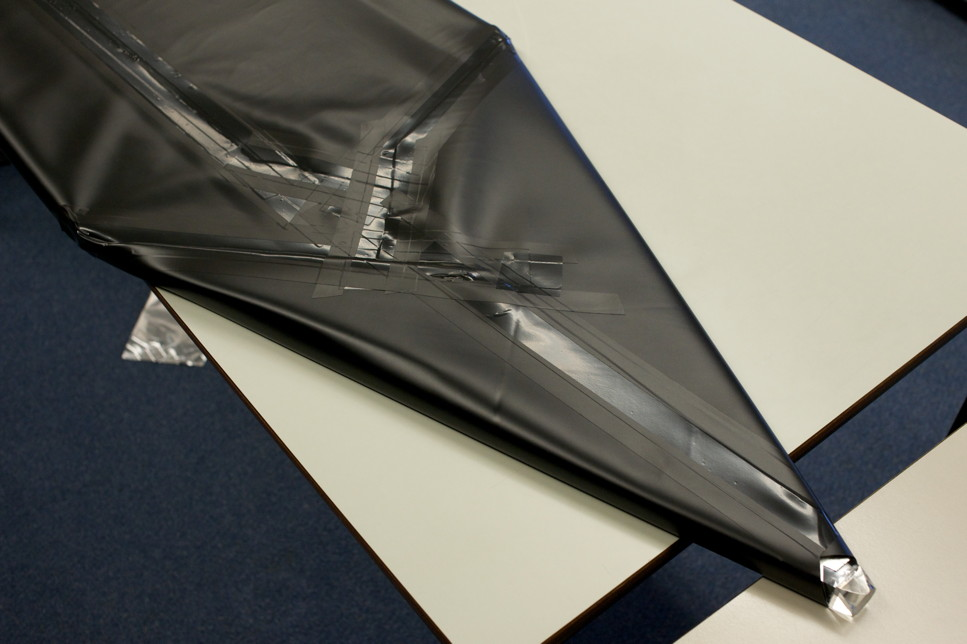
\includegraphics[width=0.47\linewidth]{vijverfolie_tape}
    \caption{De detector helemaal ingepakt, op aansluitblokje en \pmt na.}
    \label{fig:vijverfolie_tape}
\end{figure}


\section{\pmt bevestigen}

\textbf{Let op!} De \pmt NOOIT zonder beschermfolie aansluiten op de
elektronica of voeding.

% FIXME: In ander document beschrijven hoe de PMT ijking werkt?
% De \pmt moet eerst worden geijkt!
Oefen eerst voordat je de beschermfolie van de \pmt afhaalt.

\begin{enumerate}
    \item Maakt de te plakken oppervlaktes schoon et alcohol, het
    venster van de \pmt en de bovenkant van het aansluitblokje. Laat het
    alcohol verdampen voordat je begin met plakken.
    \item Knip een stukje van de optische tape af dat groot genoeg is
    voor de \pmt.
    \item Plak dit stukje bovenop het aansluitblokje zo dat er geen
    luchtbellen onder zitten. Snij of knip het overtollige tape weg. Zie
    \figref{fig:optisch_tape}.
    \item Verwijder het beveiligingsfolie van de voorkant van de \pmt.
    \item Verwijder nu voorzichtig de rode bescherming aan de andere
    kant van de tape met een pincet.
    \item Bevestig de \pmt op de bovenkant van het aansluitblokje. Doe
    dit door de buis eerst aan de rand op te zetten en dan met een
    rollende beweging verder vast te maken. Op deze manier voorkom
    luchtbellen onder het plakband.
    \item Breng aluminiumfolie aan op het overgebleven stuk van de
    detector, tot net onder de \pmt.
    \item Verstevig de \pmt constructie met houten spalken, zoals te
    zien in \figref{fig:pmt_spalken}.
    \item Pak het \pmt gedeelte daarna ook in met vijverfolie en
    voldoende zwarte tape.
\end{enumerate}

\begin{figure}
    \centering
    \subfloat[]{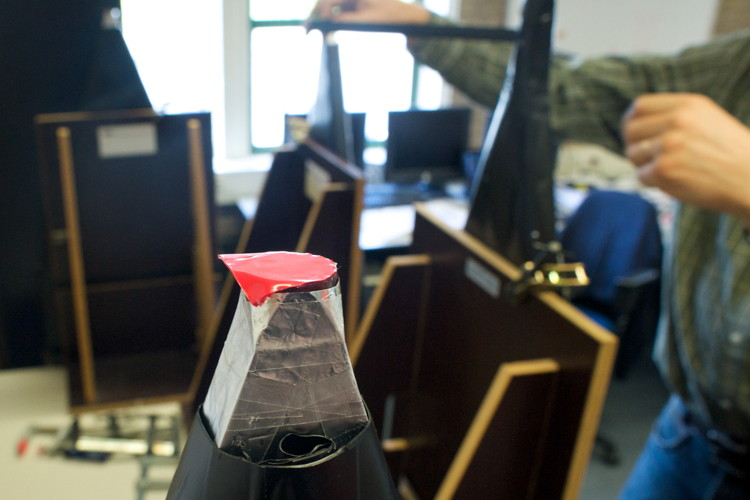
\includegraphics[width=0.47\linewidth]{optisch_tape}
                \label{fig:optisch_tape}}
    \subfloat[]{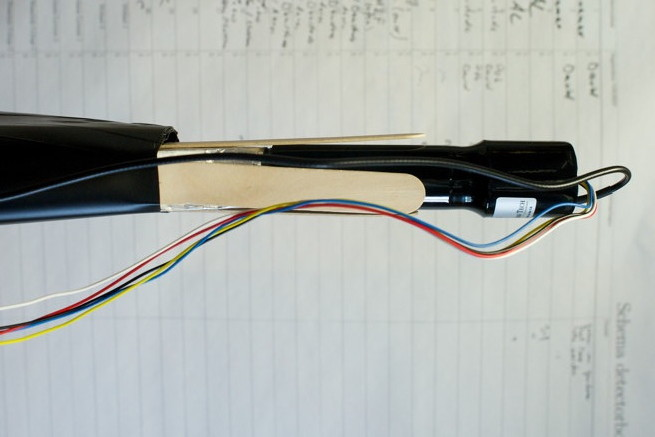
\includegraphics[width=0.47\linewidth]{pmt_spalken}
                \label{fig:pmt_spalken}}
    \caption{Optisch tape op het aansluitblokje en de \pmt bevestigd,
             met spalken ondersteund.}
\end{figure}


\section{Controleren}

Nu zou de de detector af moeten zijn. Test dit door de \pmt te verbinden
met de \hisparc elektronica die aan een pc hangt met de \hisparc
software. Stel de detector af zodat die goed is ingesteld. Zo kan je aan
aantal mogelijke problemen testen voordat de detector op het dak
geplaatst wordt. Zo zijn lichtlekken en problemen met de \pmt snel te
testen.

%\begin{thebibliography}{9}
%\end{thebibliography}

\end{document}
